% ==============================================================================
% MODULE 04: KEY FEATURES AND TECHNICAL IMPLEMENTATION
% ==============================================================================

\chapter{Key Features and Technical Implementation}
\label{chap:features_implementation}

This chapter provides an exhaustive technical analysis of CustardFin's core functional requirements (FR-1 through FR-10), demonstrating how each requirement is translated into robust software implementations. It details local ingestion, hardware-accelerated transcoding pipelines, reverse proxy NAT traversal, the Origin Shield caching mechanics, ephemeral liveness tracking, dual-path LAN/Remote routing, and presents an annotated visual walkthrough of the user interface.

% ------------------------------------------------------------------------------
\section{Local Media Organization and Private SQLite Storage (FR-1, FR-3)}
\label{sec:feat_storage}
% ------------------------------------------------------------------------------

In compliance with Invariant 8, all private media files, file system paths, cryptographic hashes, and viewer watch progress reside strictly on the user's home edge machine.

\subsection{Recursive Ingestion Scanner}
The edge daemon (\texttt{apps/edge}) incorporates a background file scanner implemented in Go (\texttt{internal/adapters/fs/scanner.go}). The scanner recursively traverses user-designated storage directories, filtering files against allowed container extensions (\texttt{.mp4}, \texttt{.mkv}, \texttt{.mov}, \texttt{.avi}, \texttt{.webm}). To eliminate duplicate transcoding jobs caused by file renaming or symbolic link aliasing, the scanner calculates a 64-bit fast signature:
\begin{equation}
    S_{\text{file}} = (\text{DeviceID} \ll 32) \oplus \text{InodeNumber}
\end{equation}
and computes a partial SHA-256 hash over the initial 64~KB container header combined with the total file size and modification timestamp. If the hash matches an existing record in the local database, the file is identified as a known asset and redundant transcode cycles are averted.

\subsection{Embedded Pure-Go SQLite Architecture}
The edge database is implemented using \texttt{modernc.org/sqlite}, a pure-Go transpiled SQLite engine that operates without CGO bindings, ensuring cross-platform static compilation. 

To guarantee concurrent read access during continuous background write operations (such as transcode progress updates and chunk indexing), the database connection initializes with high-concurrency pragmas:
\begin{lstlisting}[language=sql,caption={SQLite Edge Database Optimization Pragmas}]
PRAGMA journal_mode = WAL;
PRAGMA busy_timeout = 5000;
PRAGMA synchronous = NORMAL;
PRAGMA foreign_keys = ON;
PRAGMA temp_store = MEMORY;
\end{lstlisting}

Write-Ahead Logging (WAL) creates a separate \texttt{-wal} log file, enabling simultaneous non-blocking reads by the local streaming server while the background ingestion worker appends newly completed HLS chunks.

% ------------------------------------------------------------------------------
\section{Asynchronous Pre-Encoding and Hardware Acceleration (FR-4, FR-5)}
\label{sec:feat_transcoding}
% ------------------------------------------------------------------------------

Real-time on-the-fly transcoding incurs unacceptable latency and frequently oversubscribes residential CPU cores. CustardFin eliminates live transcoding by implementing an asynchronous pre-encoding pipeline producing standardized HTTP Live Streaming (HLS) assets.

\subsection{Adaptive Bitrate Ladder and Strict GOP Alignment}
Incoming master files are pre-encoded into an adaptive bitrate ladder conforming to RFC 8216 \cite{pantos2017http}, structured into three standard renditions:
\begin{itemize}
    \item \textbf{1080p High:} $1920 \times 1080$ resolution, $5{,}000\text{ kbps}$ target video bitrate, $192\text{ kbps}$ AAC audio.
    \item \textbf{720p Mid:} $1280 \times 720$ resolution, $2{,}800\text{ kbps}$ target video bitrate, $128\text{ kbps}$ AAC audio.
    \item \textbf{480p Low:} $854 \times 480$ resolution, $1{,}200\text{ kbps}$ target video bitrate, $96\text{ kbps}$ AAC audio.
\end{itemize}

To guarantee seamless multi-bitrate rendition switching without decoder stalls, keyframes must align across all profiles at exact segment boundaries. CustardFin enforces strict Group of Pictures (GOP) parameters in FFmpeg:
\begin{lstlisting}[language=bash,caption={FFmpeg Transcoding Command with Strict GOP Keyframe Alignment}]
ffmpeg -hide_banner -loglevel error -y -i input_master.mkv \
  -vf "scale=1920:1080:force_original_aspect_ratio=decrease,pad=1920:1080:(ow-iw)/2:(oh-ih)/2" \
  -c:v h264_nvenc -preset p4 -tune hq -b:v 5000k -maxrate 5500k -bufsize 10000k \
  -g 120 -keyint_min 120 -sc_threshold 0 \
  -c:a aac -b:a 192k -ar 48000 \
  -hls_time 4 -hls_playlist_type vod \
  -hls_segment_filename "chunks/1080p/seg_%04d.ts" \
  chunks/1080p/index.m3u8
\end{lstlisting}
The parameters \texttt{-g 120 -keyint\_min 120 -sc\_threshold 0} force an IDR keyframe precisely every 120 frames ($4.0\text{ seconds}$ at $30\text{ fps}$), preventing FFmpeg from inserting intermediate scene-change keyframes that would disrupt segment boundary synchronization.

\subsection{Hardware Probe and Fault-Tolerant CPU Fallback}
At daemon initialization, the transcoder manager (\texttt{internal/adapters/ffmpeg/transcoder.go}) executes an automated capability probe. It dynamically checks for hardware encoder acceleration using:
\begin{enumerate}
    \item \textbf{NVIDIA NVENC:} Tests \texttt{h264\_nvenc} via a synthetic 1-second test encode to GPU memory.
    \item \textbf{Intel QuickSync / VAAPI:} Tests \texttt{h264\_qsv} or \texttt{h264\_vaapi}.
    \item \textbf{CPU Fallback:} If hardware initialization fails or GPU memory is saturated, the daemon transparently defaults to the software encoder \texttt{libx264} with \texttt{-preset veryfast}.
\end{enumerate}

% ------------------------------------------------------------------------------
\section{Outbound Reverse Tunneling for CGNAT Bypass (FR-7)}
\label{sec:feat_cgnat_tunnel}
% ------------------------------------------------------------------------------

In adherence to Invariant 2, home edge nodes never require open inbound firewall ports or router UPnP configuration. Network address translation traversal across residential Carrier-Grade NAT (CGNAT) is executed via Fast Reverse Proxy (FRP) \cite{fatedier2024frp}.

\subsection{Tunnel Connection Mechanics}
The edge daemon acts as a managed parent process supervising the \texttt{frpc} child process:
\begin{enumerate}
    \item At startup, \texttt{edged} generates an ephemeral configuration binding its local HTTP streaming server (port 8089) to a designated remote virtual port on the cloud relay server (\texttt{frps}).
    \item The client initiates an outbound TCP connection to the cloud relay's public IP on port 7000 over TLS 1.3 \cite{rescorla2018transport}.
    \item A pre-shared cryptographic bearer token authenticates the node.
    \item A Yamux multiplexed session is established over the single outbound TCP connection.
\end{enumerate}
When the cloud API requires a video chunk on cache miss, it routes an internal HTTP request through the local relay port, which is transparently forwarded down the existing outbound TLS connection to the home node.

% ------------------------------------------------------------------------------
\section{Origin Shield Object Caching and URL Signing (FR-8, FR-10)}
\label{sec:feat_origin_shield}
% ------------------------------------------------------------------------------

The Origin Shield is CustardFin's primary bandwidth protection mechanism. Residential uplinks are severely constrained; streaming a 5~Mbps 1080p video directly to 10 simultaneous external viewers requires $50\text{ Mbps}$ of continuous upload bandwidth, instantly saturating home networks.

\subsection{Single-Upload Protection (Invariant 7)}
Under the Origin Shield, when multiple remote viewers simultaneously watch the same public media asset:
\begin{enumerate}
    \item Viewer 1 requests segment \texttt{seg\_0001.ts}.
    \item The Cloud API inspects the S3 cache bucket. On a cache miss, the API pulls \texttt{seg\_0001.ts} through the FRP reverse tunnel from the home edge node ($1 \times \text{segment size} \approx 2.5\text{ MB}$).
    \item The chunk is simultaneously returned to Viewer 1 and committed to the S3 bucket with an S3 Lifecycle Rule set to 24-hour expiration.
    \item Viewers 2 through 10 subsequently request \texttt{seg\_0001.ts}. The Cloud API detects a cache hit and serves the chunk directly from the S3 cache or CDN edge.
\end{enumerate}
Consequently, total residential upload bandwidth consumption for that segment remains exactly $2.5\text{ MB}$, achieving a $90\%$ upload bandwidth reduction for 10 concurrent viewers.

\subsection{HMAC-SHA256 URL Signing}
To prevent hotlinking, scraping, and unauthenticated segment distribution, all media URLs are cryptographically signed. The cloud API generates short-lived signed URLs using HMAC-SHA256:
\begin{equation}
    \sigma = \text{HMAC-SHA256}\Big(K_{\text{secret}}, \; \text{NodeID} \mathbin{\Vert} \text{MediaID} \mathbin{\Vert} \text{ChunkPath} \mathbin{\Vert} T_{\text{exp}}\Big)
\end{equation}
where $K_{\text{secret}}$ is the cloud master key and $T_{\text{exp}}$ represents the expiration UNIX timestamp (default: 300 seconds). Any request presenting an expired timestamp or modified parameter string is rejected with \texttt{HTTP 403 Forbidden}.

% ------------------------------------------------------------------------------
\section{Node Health and Ephemeral Heartbeat Liveness (FR-9)}
\label{sec:feat_heartbeat}
% ------------------------------------------------------------------------------

Distributed edge nodes operate on residential broadband connections subject to intermittent IP reassignments, router power cycles, and computer sleep states. Tracking node availability without overwhelming the cloud database is critical.

\subsection{Redis TTL Beacons}
CustardFin implements an ephemeral heartbeat mechanism:
\begin{itemize}
    \item Every 15 seconds, the edge daemon sends an authenticated beacon:
    \begin{equation}
        \text{POST } /v1/\text{nodes}/\{\text{node\_id}\}/\text{heartbeat} \quad \text{Payload: } \{\text{active\_streams}: 2\}
    \end{equation}
    \item The cloud API stores a key in Redis:
    \begin{equation}
        \text{SETEX } \texttt{heartbeat:\{node\_id\}} \quad 20 \quad \text{"alive"}
    \end{equation}
    with an exact Time-To-Live (TTL) of 20 seconds (providing a 5-second network jitter grace period).
    \item When a viewer accesses the catalog, the API checks for the existence of \texttt{heartbeat:\{node\_id\}}.
    \item If the home node powers down or suffers an ISP outage, Redis automatically evicts the key after 20 seconds. The catalog immediately marks the node as \textit{Offline}, preventing viewers from attempting failed streams.
\end{itemize}

% ------------------------------------------------------------------------------
\section{Dual-Path Streaming and Embedded Mini-Jellyfin (FR-6)}
\label{sec:feat_dual_path}
% ------------------------------------------------------------------------------

CustardFin features intelligent dual-path streaming routing based on client network proximity.

\subsection{Stream Router Proximity Resolution}
When a playback request arrives at \texttt{GET /v1/media/\{id\}/playback}, the stream router executes proximity analysis:
\begin{enumerate}
    \item It extracts the requesting client's IP address ($IP_{\text{client}}$).
    \item It compares the client's public NAT IP and subnet against the node's registered LAN IP.
    \item \textbf{LAN Match:} If the client resides on the identical local area network as the edge node (e.g., both within \texttt{192.168.1.0/24}), the API returns a direct LAN streaming endpoint:
    \begin{equation}
        URL_{\text{play}} = \texttt{http://192.168.1.105:8089/hls/1080p/index.m3u8}
    \end{equation}
    The client streams directly from the home machine at full gigabit Ethernet/Wi-Fi speeds with zero cloud egress cost and sub-second start latency.
    \item \textbf{Remote Match:} If the client is external, the API routes the request through the Origin Shield cache path.
\end{enumerate}

\subsection{Embedded Mini-Jellyfin Standalone Hub}
To guarantee full functionality during cloud outages or internet severance, the edge daemon embeds a standalone offline single-page application (\texttt{embedded\_ui.go}) directly inside the Go binary. Serving on port \texttt{8089}, the Mini-Jellyfin hub enables users on the local network to:
\begin{itemize}
    \item Search and browse the complete local media library directly from SQLite.
    \item Stream high-bitrate multi-channel audio and video via native HLS.js.
    \item Manage local file ingestion and monitor NVENC hardware encoder health.
\end{itemize}

% ------------------------------------------------------------------------------
\section{User Accounts, Edge Node Claiming, and Video Management}
\label{sec:feat_auth_claiming}
% ------------------------------------------------------------------------------

CustardFin enforces secure multi-tenant isolation across all control operations.
\begin{itemize}
    \item \textbf{User Authentication:} Implements JSON Web Tokens (JWT) signed via HMAC-SHA256 with 15-minute access tokens and 7-day refresh tokens. Passwords are cryptographically hashed using \texttt{argon2id} with memory cost $64\text{ MB}$, time cost 3 iterations, and 4 parallelism threads.
    \item \textbf{Node Claiming Handshake:} When a new edge node starts, it generates a unique hardware node UUID and a one-time cryptographic claim challenge. The user logs into the web dashboard and claims the node via \texttt{POST /v1/nodes/claim}. Once claimed, the node is cryptographically bound to that user's account, preventing unauthorized remote access or manifest spoofing.
    \item \textbf{Public / Private Manifest Sync:} Users toggle media visibility with a single click. When set to Private, all metadata remains exclusively in local SQLite. When toggled to Public, the edge daemon syncs a lightweight 650-byte JSON manifest to PostgreSQL, registering the title in the global community feed.
\end{itemize}

% ------------------------------------------------------------------------------
\section{User Interface Walkthrough with Screenshots}
\label{sec:feat_screenshots}
% ------------------------------------------------------------------------------

This section provides comprehensive visual documentation of CustardFin's user experience across both the cloud presentation tier and the embedded edge interfaces.

\subsection{Community Catalog Feed}
Figure~\ref{fig:ui_catalog_feed} illustrates the public community catalog rendered via Next.js React Server Components. The feed displays discoverable titles hosted across active home nodes, featuring real-time node availability indicators, duration badges, and uploader attribution.

\begin{figure}[htbp]
\centering
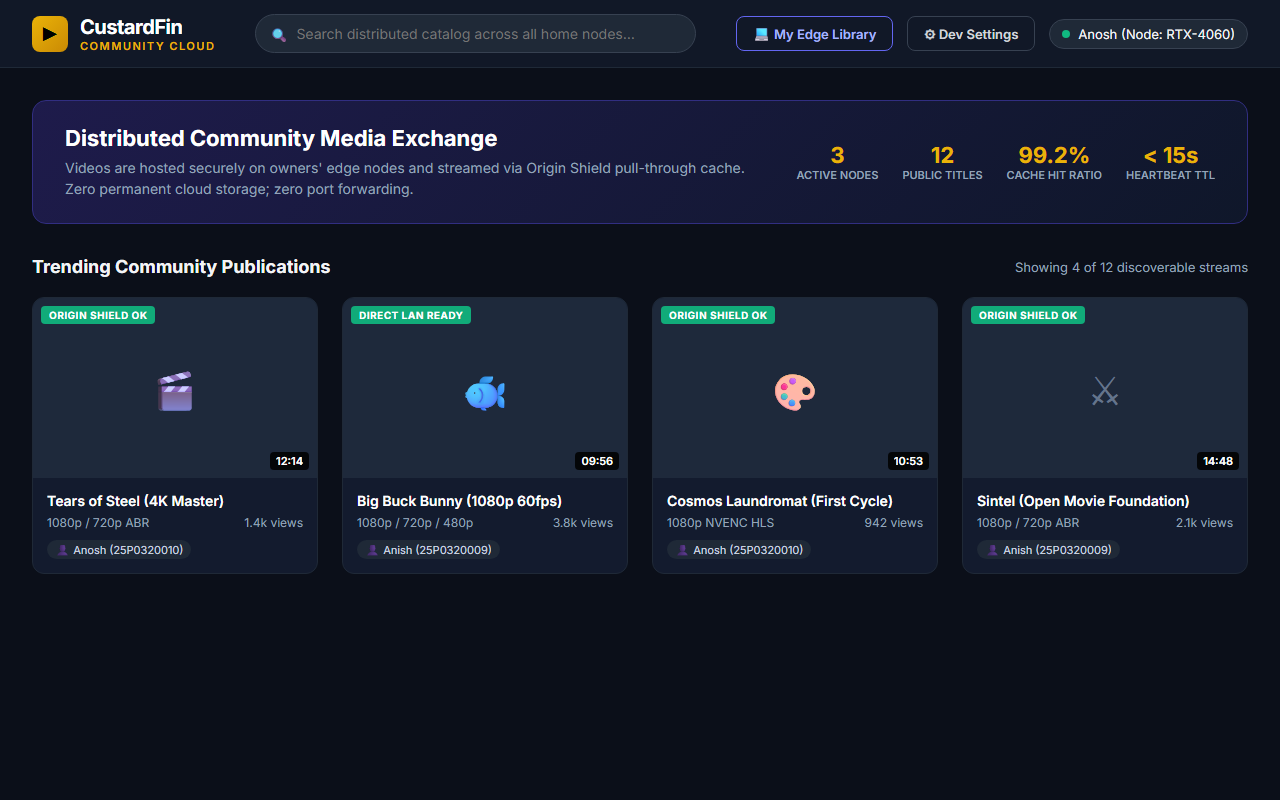
\includegraphics[width=0.95\textwidth]{figures/ui_catalog_feed.png}
\caption{CustardFin Community Catalog Feed: Distributed Discovery and Real-Time Node Status}
\label{fig:ui_catalog_feed}
\end{figure}

\subsection{Video Player with ``Stats for Nerds'' HUD}
Figure~\ref{fig:ui_player_stats} depicts the high-definition video player operating with the engineering telemetry overlay (``Stats for Nerds'') active. The HUD provides live inspection of video resolution, HLS segment duration, buffer health, active delivery path (S3 Origin Shield cache hit), and signed URL expiration.

\begin{figure}[htbp]
\centering
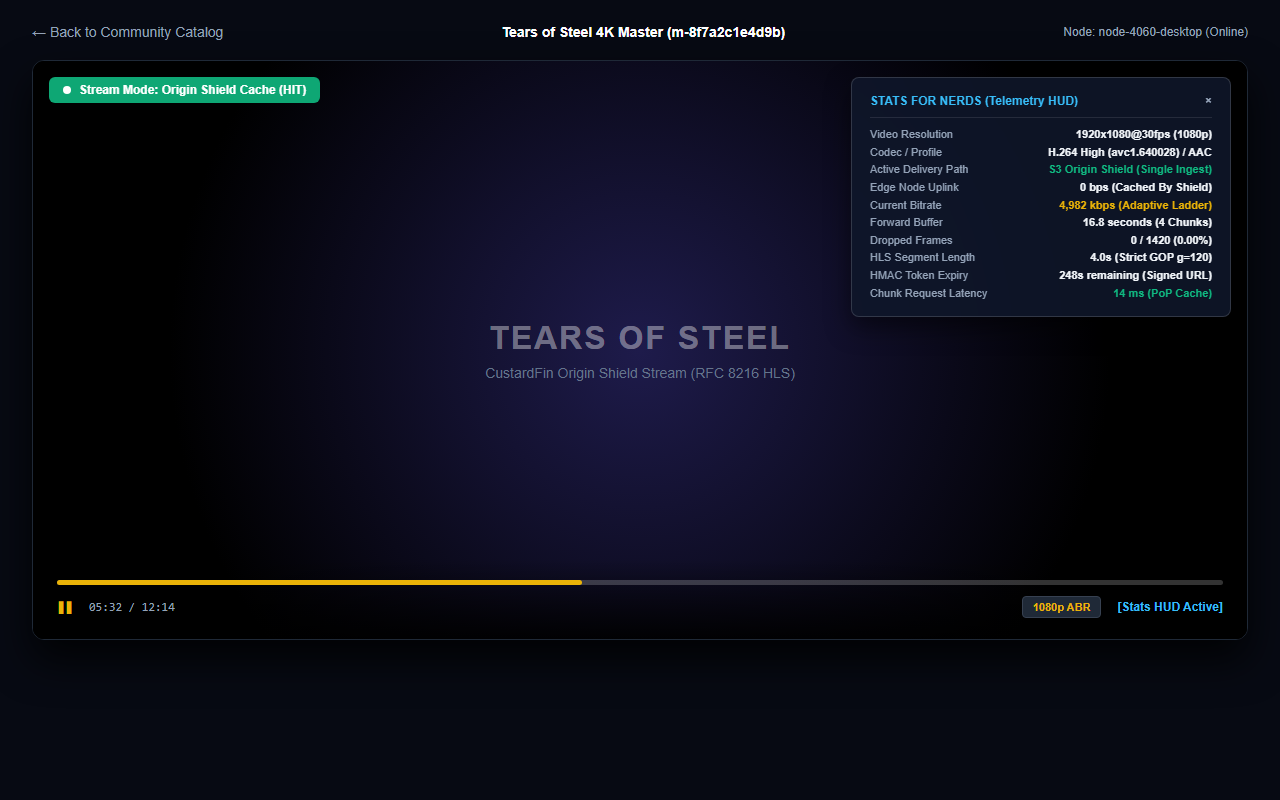
\includegraphics[width=0.95\textwidth]{figures/ui_player_stats.png}
\caption{Video Player Interface with Real-Time ``Stats for Nerds'' Engineering Telemetry HUD}
\label{fig:ui_player_stats}
\end{figure}

\subsection{My Edge Library Manager}
Figure~\ref{fig:ui_edge_library} shows the Edge Library Manager modal. From this interface, node owners inspect local hardware transcode capabilities (NVIDIA NVENC active), monitor local storage consumption, toggle public/private manifest synchronization, and initiate direct LAN playback sessions.

\begin{figure}[htbp]
\centering
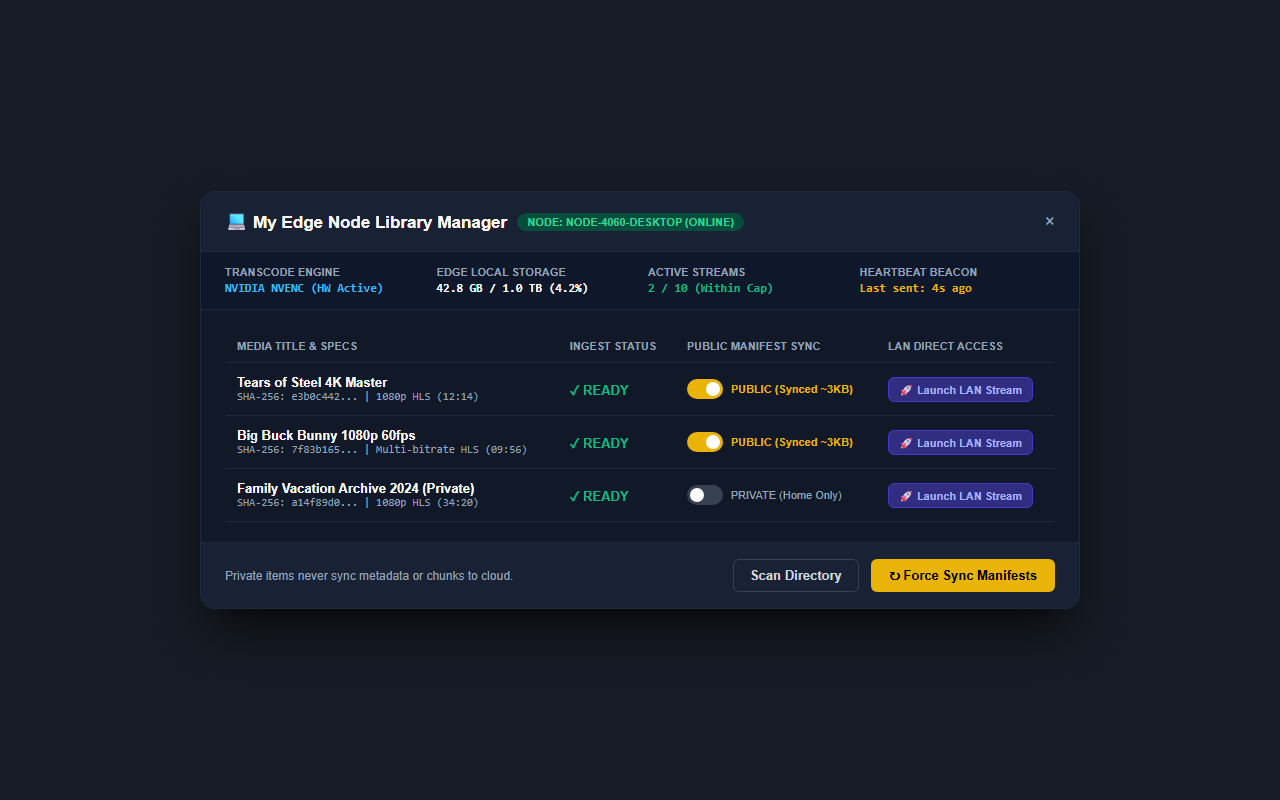
\includegraphics[width=0.95\textwidth]{figures/ui_edge_library.png}
\caption{My Edge Library Modal: Node Management, Storage Quota, and Public/Private Toggles}
\label{fig:ui_edge_library}
\end{figure}

\subsection{Embedded Standalone Mini-Jellyfin Hub}
Figure~\ref{fig:ui_mini_jellyfin} displays the offline Mini-Jellyfin web portal served directly by the Go edge daemon on port 8089. It operates with zero cloud dependencies, enabling local LAN media playback even when external internet connectivity is completely severed.

\begin{figure}[htbp]
\centering
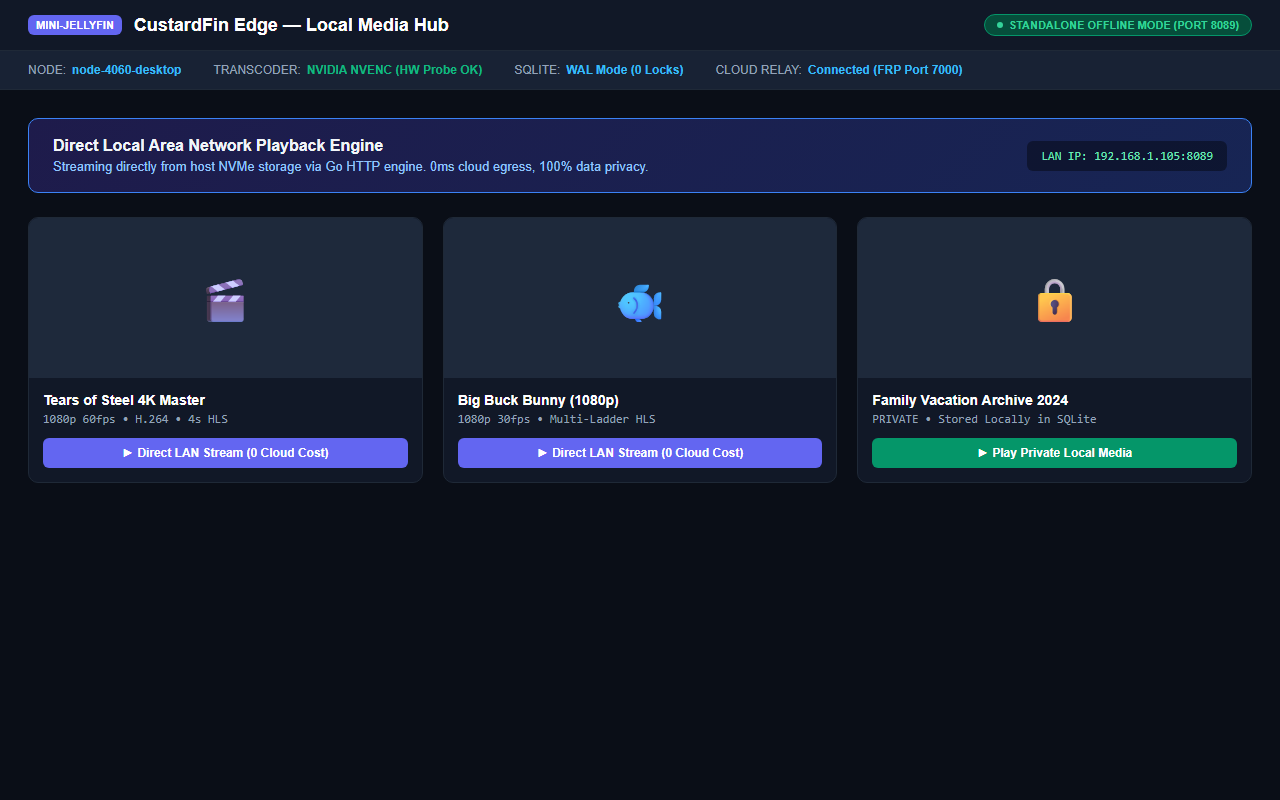
\includegraphics[width=0.95\textwidth]{figures/ui_mini_jellyfin.png}
\caption{Standalone Embedded Mini-Jellyfin Offline Web Hub (Port 8089 Direct LAN Streaming)}
\label{fig:ui_mini_jellyfin}
\end{figure}

\subsection{Developer Settings and Diagnostics Modal}
Figure~\ref{fig:ui_dev_settings} illustrates the developer diagnostics and grading topology configuration interface. It provides hot-reconfigurable API endpoints, S3 cache emulators, and active admission limiter status verification.

\begin{figure}[htbp]
\centering
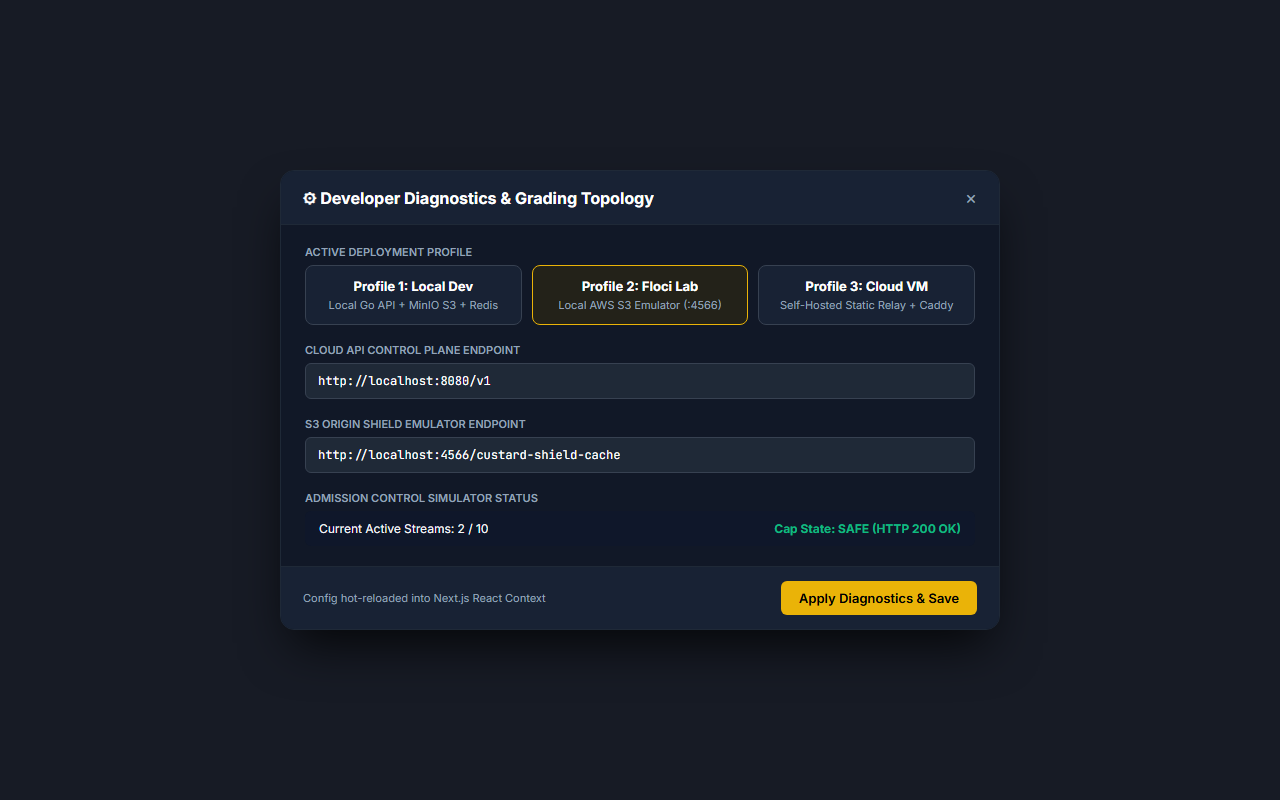
\includegraphics[width=0.92\textwidth]{figures/ui_dev_settings.png}
\caption{Developer Diagnostics and Grading Topology Configuration Interface}
\label{fig:ui_dev_settings}
\end{figure}
